\documentclass{article}
\usepackage{graphicx}
\usepackage{ragged2e}
\usepackage{geometry}
\title{Experimentation}
\author{Vigneswaran Chandrasekaran}
\date{10-11-2019}

\begin{document}
\flushleft{\huge{\textbf{Discussions}}}
\section{Discussions}
The goal of this research article is to develop a parochial pre-training model which
initializes near optimal parameters by forming bins based on the MI between the input
data and the neuron activations. Further, the number of bins was selected using partial
information decomposition and the parameters were updated using the novel weight
update rule during pre-training. This way of pre-training ensures the high possibility of
reaching the near global optimal position. To show the supremacy of the proposed model
in terms of stability, convergence rate, the comparisons were made with state-of-the-art
weight initialization methods and pre-training techniques.

\subsection{Comparison with other Weight Initialization methods}
To check how effective the parameters obtained from unsupervised bin-wise pre-training
model can effectively locate the model near to the potential local minima and results to
faster convergence, the proposed work was compared with various Weight Initialization
methods. Well-known and effective Weight initialization methods including Xavier [43],
Kaiming [44] and Orthogonal methods [42] were taken into account for comparison. All the weight initialization methods were configured with default parameter values as mentioned in Pytorch's torch.nn.init module to make the results obtain more reliable.

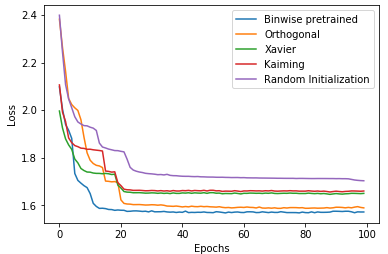
\includegraphics[width= 7cm, height=5cm]{fig1.png}
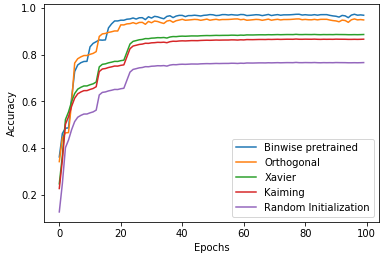
\includegraphics[width= 7cm, height=5cm]{fig2.png}
\\
Fig 7(a) \& Fig 7(b) shows the validation loss and Validation accuracy of various Weight Initialization methods for MNIST dataset respectively
\\
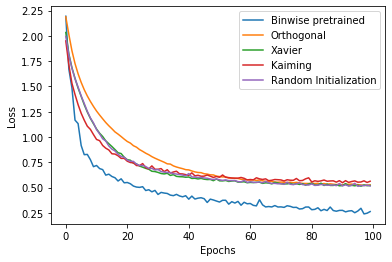
\includegraphics[width= 7cm, height=5cm]{fig5.png}
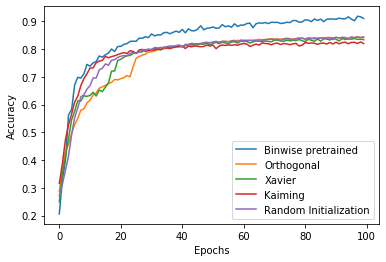
\includegraphics[width= 7cm, height=5cm]{fig6.png}
\\
Fig 8(a) \& Fig 8(b) depicts the validation loss and Validation accuracy of various Weight Initialization methods for Fashion MNIST dataset respectively
\\
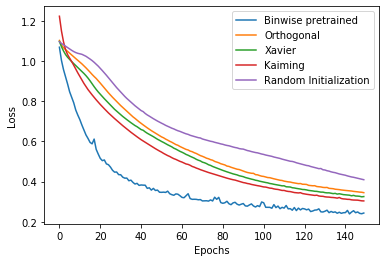
\includegraphics[width= 7cm, height=5cm]{fig3.png}
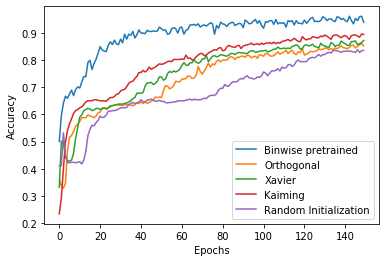
\includegraphics[width= 7cm, height=5cm]{fig4.png}
Fig 9(a) \& Fig 9(b) plots the validation loss and Validation accuracy of various Weight Initialization methods for University of Bern EEG dataset respectively
Figure 7, 8 and 9 shows clear dominance of the proposed binwise pretraining method.

\end{document}